% !TEX root = ../../main.tex
% !TEX encoding = UTF-8 Unicode
%%%
\chapter{The Standard Model}
\label{ch:stdmodel}

% Inline fraction for text
%\newcommand{\slantfrac}[2]{\,^#1\!/_#2}


The Standard Model (SM) is a quantum field theory describing the elementary particles and fundamental forces (with the exception of gravity)
%\footnote{Except when stated otherwise, discussion of forces in the context of the SM will not refer to gravity.} 
that govern the universe. At its core, the SM states that all matter is composed of fundamental particles called fermions, all forces are mediated by force carrying gauge bosons, and all massive fundamental particles acquire their mass through interactions with the Higgs boson.

The importance of the SM to our understanding of the physical world is reflected in the 17 Nobel Prizes in physics that have been awarded since 1957 for work relating to the development and verification of the SM~\cite{Nobel_Prizes}. That the current theory describes with remarkable accuracy nearly all observed phenomena of electromagnetic, weak, and strong interactions in a compact theory with rich symmetries can belie the tumultuous and often uncertain path that lead to it's development. In this chapter, a brief discussion of the content and formulation of the SM is presented. 

%
\section{Particle Content}

In ~\Fig{\ref{fig:st_m_p}}, the particle content of the SM is succinctly summarized. The particles are elementary: they cannot be decomposed further into smaller constituents. There are two broad categories of particles: fermions (half integer spin) and bosons (integer spin). Spin is an intrinsic property of a particle, and is a form of angular momentum. Fermions and bosons necessarily behave differently according to the Spin-Statistics Theorem\footnote{
	An important consequence of the theorem is the Pauli exclusion principle for fermions: no two fermions can occupy the same quantum state. Bosons have no such restriction, and thus any number can occupy the same quantum state.
}~\cite{spin_stats}. The fermions in the SM are further subdivided into quarks and leptons, while the bosons are subdivided into gauge (spin 1) and scalar (spin 0) bosons. 

\begin{figure}[htb]
\begin{center}
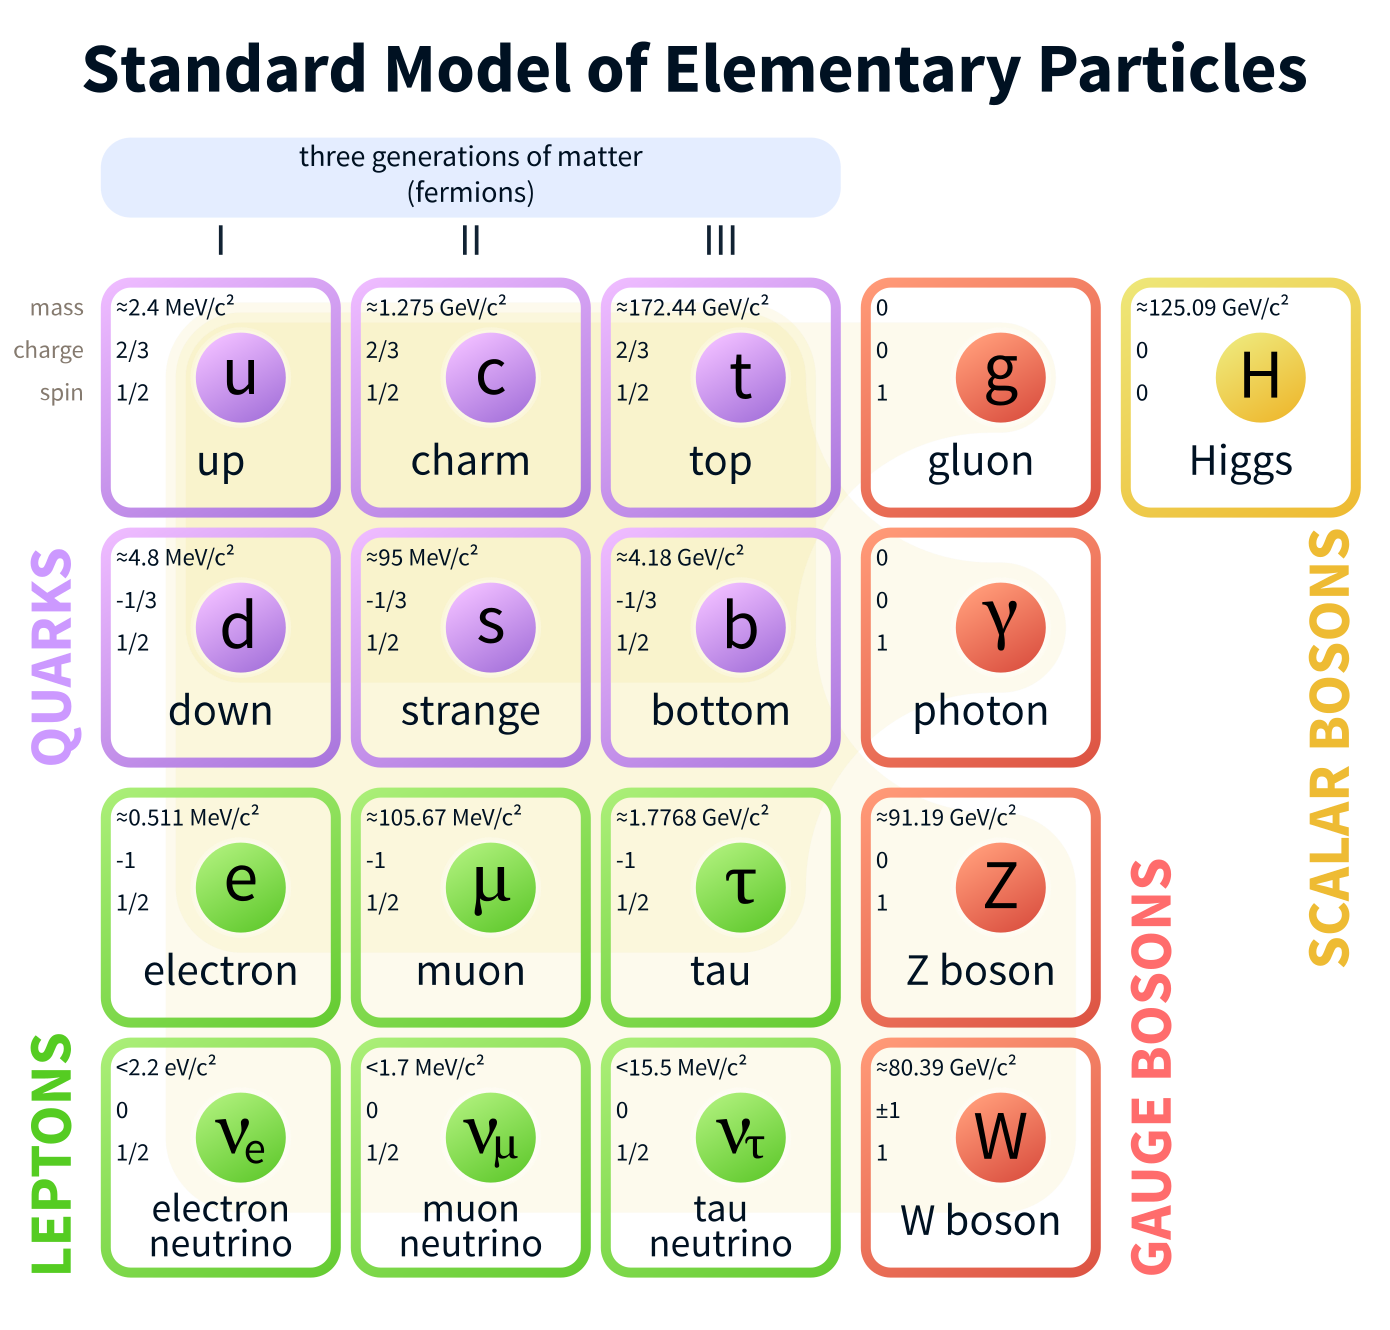
\includegraphics[width=0.7\textwidth]{figures/StandardModel/std_model}
\end{center}
\caption[Fundamental particles in the Standard Model]{A categorization of the fundamental particles in the Standard Model is shown: quarks and leptons together constitute all the matter particles, the gauge bosons mediate the electromagnetic, weak, and strong forces, and the Higgs boson generates mass for the fundamental particles.}
\label{fig:st_m_p}
\end{figure}

All matter is composed of quarks and leptons, which are divided into three generations of increasing mass\footnote{
	The exact mass hierarchy of the neutrinos has not been determined.
}. A generation includes two quarks, one with electric charge $+2/3$ (in units of the fundamental electric charge scale, $e$) and one with $-1/3$, one negatively charged lepton, and one neutral lepton called a neutrino. The particles in different generations mainly differ in their masses. Each fermion has an associated anti-particle with identical properties, with the exception of an inverted electric charge.

The three quarks with electric charge $+2/3$, known as up-type quarks, are called up, charm, and top, and are denoted by u, c, and t, respectively. The three quarks with electric charge $-1/3$, known as down-type quarks, are called down, strange, and bottom, and are denoted by d, s, and b, respectively. Due to the strong force, quarks do not exist in isolation, but rather combine to form hadrons like protons, neutrons, and pions. Hadrons are typically composed of either two quarks (meson) or three quarks (baryon), although a pentaquark state has been recently experimentally verified~\cite{pentaquark}.

In order of increasing mass, the charged leptons are the electron, muon, and tau and are denoted by $e,\mu$, and $\tau$, respectively. The neutrinos are labeled by the charged lepton in their generation: $\nu_e,\nu_{\mu}$, and $\nu_{\tau}$. 
Leptons only interact with the electromagnetic and weak forces, and in contrast to quarks can exist in isolation. The heaviest charged leptons have a finite lifetime and decay to electrons which are stable. Neutrinos have an extremely small, non-zero mass, and oscillate as they propagate through space\footnote{
	The oscillation is a predictable, periodic transformation between the three neutrino generations. Neutrinos are produced in weak eigenstates, e.g. $\nu_e$, which, however, do not correspond to mass eigenstates.
}. 

The gauge bosons mediate the electromagnetic, weak, and strong forces: particles that interact via a certain force do so through the exchange of gauge bosons. The photon has no mass or electric charge, and mediates the electromagnetic force. Since it has no mass, the photon is stable and can propagate through space indefinitely. The weak force is mediated by the $Z^0$, $W^+$, and $W^-$ bosons, where the superscript denotes the electric charge. All three weak bosons are massive, and have a finite lifetime. The gluon is responsible for mediating the strong force. Like the photon, it is massless and has no electric charge; however, it has an analogous ``color charge'' associated with the strong interaction. 

Finally, the Higgs boson is a massive scalar (spin-0) particle with no electric charge. Through a process called the Higgs mechanism, it is responsible for generating masses of the fermions, weak gauge bosons, and itself.  


%
%%%
\iffalse
%%%
\section{Arriving at the Standard Model}

Our current understanding of the fundamental interactions between elementary particles is derived from this astonishingly nascent theory. In the span of 13 years, the SM in its current form was developed. In 1961, Glashow first proposed a way to combine the electromagnetic and weak interactions~\cite{Glashow:1961tr}; in 1967, Weinberg and Salam independently incorporated the Higgs mechanism~\cite{Weinberg,Salam:1968rm}; and by 1974, quantum chromodynamics (QCD) with the inclusion of asymptotic freedom~\cite{Gross_Wilczek, Politzer} rendered the basic form of the current Standard Model\footnote{
	There would still be much to verify and refine, such as the number of leptons and quarks, but the pillars of the theory were formed. 
}. 

A mere 64 years prior to Glashow's electroweak proposal, the {\em first} fundamental particle was discovered by J.J. Thompson in 1897: the electron\footnote{
	The celerity with which this feat has been achieved is reminiscent of the 66 years separating the Wright brothers' initial flight (1903) and the Apollo 11 moon landing (1969), coincidentally transpiring nearly contemporaneously.
}. By 1911 Rutherford had discovered the nucleus and in 1913 the primitive Bohr model gave accurate predictions for Hydrogen energy levels. Even during this relatively simple period, there were hints of a coming quantum model: in 1905 Einstein's photoelectric effect unequivocally demonstrated the existence of the massless photon. 

With the advent of quantum mechanics in 1925, the picture of fundamental particles began to expand. In 1928 Dirac postulated the existence of the positron\footnote{
	He recognized his equation permitted negative energy electron solutions.
}, in 1930 Pauli theorized the neutrino to conserve energy in $\beta$ decays, and in 1935 Yukawa theorized nuclei were held together by a nuclear force through the exchange of mesons.  

In 1947, most of the predicted particles had been found\footnote{
	The muon was not predicted, but found nonetheless, while the neutrino would't be found until later.
}, however the discovery of a new meson, the kaon, would spark another revolution in the theory of elementary particles. In the following decade, a ``zoo'' of new mesons and baryons were discovered, and physicists struggled to find a way to neatly classify them. Finally in 1961, Gell-Mann introduced the Eightfold Way to describe the symmetries of mesons and baryons as representations of the group SU(3). The power of this classification of symmetries was immediately evident when the $\Omega^-$ baryon predicted by the theory was discovered in 1964. In the same year, Gell-Mann and Zweig proposed the quark model which codified the symmetries of the Eightfold Way with three quarks and anti-quarks that combined to form mesons and baryons. The use of group theory to classify the interactions of elementary particles in terms of symmetries would drive the development of the field, resulting eventually in the current theory of the SM.

%%%
\fi
%%%

%
\section{Formulation of Symmetries}
The principle of least action with a Lagrangian density is used to describe the propagation and interactions of quanta and fields: for an arbitrary field $\phi$, obeying the equations of motion described by the Lagrangian density, $\mathcal{L}(\phi,\partial \phi)$, the action is defined as:
 $$S[\phi] = \int d^4x \mathcal{L}(\phi(x),\partial\phi(x)); \quad\quad \delta S = 0$$ 
 According to Noether's Theorem, for every continuous global symmetry of the action, there is an associated conserved charge~\cite{noether}. For local gauge symmetries, an equation of motion for generated gauge fields is produced.

The group corresponding to all Poincar\'e transformations characterizes the 10 global continuous symmetries of special relativity; translations in space and time (four), rotations in space (three), and boosts in space (three)~\cite{Srednicki}. As a relativistic quantum field theory, the SM incorporates special relativity; hence, the Poincar\'e symmetry is a global continuous symmetry of the theory. Associated with this global symmetry are three conserved quantities: energy, momentum, and angular momentum.  In the SM, spin-0 particles are described by scalar fields, $\phi$, obeying the Klein-Gordon equation, spin-$1/2$ particles are described by spinor fields, $\psi$, obeying the Dirac equation, and spin-1 particles are described by vector fields, $A_{\mu}$, obeying the Proca equation.

To impose a specific symmetry on the theory, the goal is to derive a Lagrangian which is invariant under the corresponding transformations. Often these are continuous symmetries which can be thought of as abstract rotations of the fields. As an example, consider the free spinor field obeying the Dirac equation:
$$\mathcal{L}=\bar{\psi}(\gamma^{\mu}\partial_{\mu}-m)\psi$$
This is invariant under the global transformation $\psi(x)\ra\psi'(x)=e^{i\alpha}\psi(x)$. The continuous symmetry is characterized by its infinitesimal behavior near the identity transformation. In group theory, this symmetry is characterized by the Lie algebra of U(1), for which there is one generator, $\alpha$~\cite{wukitung}. If $\alpha$ is a function of space-time, the derivative in the Lagrangian produces an extra term. To retain invariance, a covariant derivative can be introduced:
$$\partial_{\mu}\rightarrow D_{\mu} = \partial_{\mu} - ieA_{\mu}$$
where $e$ describes a coupling, and the gauge field, $A_{\mu}(x)$, transforms as:
$$A_{\mu}(x)\ra A'_{\mu}(x)=A_{\mu}(x)+ \frac{1}{e}\partial_{\mu}\alpha(x)$$
Finally, a term corresponding the the free propagation of this new massless gauge field is added to the Lagrangian.

This process of identifying a global symmetry of free fields and requiring it to also be a local or gauge symmetry is the general process through which the interactions in the SM are constructed. For each underlying local symmetry there are generators which form a basis for the Lie algebra describing it, and for each generator a gauge field must be introduced to preserve the symmetry. The gauge fields couple to the original fields and determine the interactions of the theory. The resulting theory is known as a gauge theory which, as shown by 't Hooft, implies the theory is renormalizable~\cite{thooft}. The full local gauge symmetry of the SM is described by the group $SU(3)\times SU(2)_L\times U(1)_Y$ which describes the strong and electroweak interactions~\cite{Griffiths, Srednicki}.

%
\section{Electroweak Sector}
The electroweak interaction preserves the internal weak isospin and weak hypercharge symmetries corresponding to the group $SU(2)_L\times U(1)_Y$. The subscript $L$ indicates that the weak isospin $SU(2)$ symmetry is restricted to left-handed fields, while the subscript $Y$ corresponds to the weak hypercharge which generates the U(1) symmetry. The electroweak interaction is thus described by a chiral theory since it couples differently to left-handed and right-handed fields, which are defined by how they behave under Lorentz transformations.

The restricted Lorentz group is a subgroup of the Poincar\'e group corresponding to the generators of boosts and rotations. These six generators can be rearranged into a direct sum of two Lie algebras corresponding to the group $SU(2)\times SU(2)$~\cite{Srednicki}. A fermion field can be expressed as a Dirac spinor in the $(\frac{1}{2},0)\oplus(0,\frac{1}{2})$ representation of the restricted Lorentz group as $\Psi = \begin{pmatrix}\psi_L\\\psi_R\end{pmatrix}$, where $\psi_L$ and $\psi_R$ are left-handed and right-handed Weyl spinors. The left-handed and right-handed spinor components of the Dirac field do not mix under a Lorentz transformation.

The chiral, weak isospin symmetry is maximally parity violating: left handed fermion fields transform as $SU(2)_L$ doublets in the defining representation, while right-handed fermion fields are represented as $SU(2)_L$ singlets in the trivial representation. The lepton and quark fields can be grouped in terms of their chiral components as shown in~\Tab{\ref{tab:ew_rep}}.  There are three generators for the Lie algebra of $SU(2)$; thus, by requiring $SU(2)_L$ to be a local gauge symmetry, three vector gauge fields are introduced in the adjoint representation: $W_{\mu}^1,W_{\mu}^2$, and $W_{\mu}^3$. 

The $U(1)_Y$ weak hypercharge symmetry is not chiral, as it couples to both left-handed and right-handed fields. The weak hypercharge of a field is chosen in a suggestive way: $Y=2(Q-I_3)$, where $Q$ is the electric charge and $I_3$ is the third component of the weak isospin. Corresponding to the single generator of the Lie algebra of $U(1)$, one vector gauge field, $B_{\mu}$, is introduced to ensure the local gauge invariance of the $U(1)_Y$ symmetry. 

\begin{table}[tbp]
\begin{center}
\begin{tabular}{lccc}
\hline\hline
Particle type & SU(2)$_L$ Grouping & Isospin ($I_3$) & Hypercharge (Y) \\\hline
Left-handed leptons &$ \begin{pmatrix} \nu_L \\ e_L \end{pmatrix} $& $\pm\frac{1}{2}$ &$ -1$\\
Left-handed quarks &$ \begin{pmatrix} u_L \\ d_L \end{pmatrix} $& $\pm\frac{1}{2}$ &$ \frac{1}{3}$\\
Right-handed neutrino$^{\dagger}$& $\nu_R$ & 0 & 0 \\
Right-handed electron & $e_R$ & 0 & $-2$ \\
Right-handed up quark & $u_R$ & 0 & $\frac{4}{3}$\\
Right-handed down quark & $d_R$ & 0 &$-\frac{2}{3}$\\\hline\hline
\end{tabular}
\end{center}
\caption[Weak isospin and hypercharge groupings of the electroweak sector]{The weak isospin and hypercharge properties of the first generation of fermions is presented.\\\,$^{\dagger}$Right-handed neutrinos do not interact at all, if they exist. For this reason they are not usually included in the formulation of the SM.}
\label{tab:ew_rep}
\end{table}

The four vector gauge fields $W_{\mu}^i, B_{\mu}$ and all the fermion fields must be massless to preserve the imposed gauge invariance; however, experimentally all fermions have mass, and there are three massive weak bosons and one massless photon. The solution is to introduce a complex scalar field, $\Phi=\begin{pmatrix}\phi^+\\\phi^0\end{pmatrix}$, which is a weak isospin doublet with hypercharge $Y=1$, and a potential of the form $V(\Phi) = -\mu^2\Phi^{\dagger}\Phi + \lambda(\Phi^{\dagger}\Phi)^2$, which furthermore respects gauge invariance. By expanding the field about the minimum of the potential, known as the vacuum expectation value $v$, and choosing the unitary gauge so that it is real, the scalar field becomes $\Phi=\frac{1}{\sqrt{2}}\begin{pmatrix}0\\v+H(x)\end{pmatrix}$. The excitation field, $H$, is now interpreted as the physical Higgs field, and the constant, non-zero vacuum expectation value will introduce mass terms for the gauge fields.

The settling of the complex field into the non-zero minimum of the potential, $v$, is known as spontaneous symmetry breaking. By Goldstone's theorem, there should be three massless bosons corresponding to the generators of the spontaneously broken continuous global symmetry~\cite{Goldstone,gold_salam_wein}. By using gauge invariance to select the unitary gauge, however, the three degrees of freedom corresponding to the Goldstone bosons are recast as longitudinal polarizations of the now massive $W^{\pm}_{\mu}$ and $Z_{\mu}^0$ gauge bosons. The combination of spontaneous symmetry breaking with gauge invariance to endow mass to vector gauge fields is called the Higgs mechanism~\cite{brout_englert,higgs_mech,gur_hag_kib}. The fermions can now also acquire mass through added Yukawa couplings of the Dirac fermions to the scalar $\Phi$.

The mass eigenstates of the vector gauge fields can be expressed in terms of the original gauge fields as shown in~\Eqns{\ref{eq:az_mix}}{\ref{eq:w_mix}}.
\begin{equation}
\begin{pmatrix}A_{\mu}\\Z_{\mu}^0\end{pmatrix}  =  \begin{pmatrix}\cos\theta_W&\sin\theta_W\\-\sin\theta_W&\cos\theta_W\end{pmatrix}\begin{pmatrix}B^0_{\mu}\\W^3_{\mu}\end{pmatrix}
\label{eq:az_mix}
\end{equation}
\begin{equation}
\label{eq:w_mix}
W^{\pm}_{\mu} = \frac{1}{\sqrt{2}}\left(W^1_{\mu}\mp iW^2_{\mu}\right)
\end{equation}
The Weinberg weak mixing angle, $\theta_W$, also relates the masses of the neutral weak vector boson, $Z_{\mu}^0$, and the charged weak vector bosons, $W^{\pm}_{\mu}$: $M_W=\cos\theta_WM_Z$. The photon field, $A_{\mu}$, remains massless, corresponding to the unbroken $U(1)_{em}$ symmetry. The electroweak and Higgs bosons after electroweak symmetry breaking are summarized in~\Tab{\ref{tab:ew_bosons}}.

\begin{table}[tbp]
\begin{center}
\begin{tabular}{lcrrr}
\hline\hline
Boson & Type &Isospin ($I_3$) & Hypercharge (Y) & Mass [\GeV]\\\hline
$W^{\pm}_{\mu}$ & Vector Gauge&$\pm 1$ & 0 & 80.4 \\
$Z^0_{\mu}$ & Vector Gauge & 0 & 0 & 91.2\\
$A_{\mu}$ & Vector Gauge& 0 & 0 &  0\\
$H^0$ & Scalar &$-\frac{1}{2}$&1 & 125.1\\\hline\hline
\end{tabular}
\end{center}
\caption[Properties of electroweak and Higgs bosons]{Properties of the electroweak gauge bosons and scalar Higgs boson after electroweak symmetry breaking are shown. The three weak vector gauge bosons acquire mass, while the photon remains massless, corresponding to the unbroken $U(1)_{em}$ symmetry.}
\label{tab:ew_bosons}
\end{table}

The massless, force-mediating photon reproduces the infinite range of electromagnetism, and interacts with particles with electric charge. The short range of the weak force is reproduced by the massive, force-mediating weak bosons. The $Z^0_{\mu}$ boson is associated with fermion-antifermion annihilation or creation, while the $W^{\pm}_{\mu}$ bosons allow for fermions to change flavor, provided the net change in electric charge of the interaction is $\Delta Q = \pm1$. For leptons, the flavor changing must involve a charged lepton and a neutrino of the same type (e.g. $e$ and $\nu_e$); however, for quarks, there is a non-zero probability for intergenerational mixing\footnote{
	An analogous flavor changing neutral current does not exist at tree level, and is suppressed even in loop diagrams.
}. The intergenerational mixing in the quark sector is characterized by the unitary CKM matrix~\cite{Cabibbo, kob_mas}\footnote{
	Similar to the neutrinos, the weak interaction eigenstates of the quarks do not correspond to the freely propagating mass eigenstates.
}. The Higgs boson allows left chiral fermion states to mix with right chiral fermion states. The SM interactions of the electroweak bosons and the Higgs boson are shown in~\Figs{\ref{fig:feyn_weak}}{\ref{fig:feyn_higgs}}.
\begin{figure}[htbp]
\begin{center}
\feynmandiagram [baseline=(d.base), horizontal=d to b] {
a[particle={\(\nu_L\)}] -- [fermion] b -- [fermion] c [particle={\(e_L\)}],
b -- [boson] d [particle=\(W^-\)], };
\feynmandiagram [baseline=(d.base), horizontal=d to b] {
a[particle=\(d_L\)] -- [fermion] b -- [fermion] c [particle=\(u_L\)],
b -- [boson] d [particle=\(W^+\)], };
\feynmandiagram [baseline=(d.base), horizontal=d to b] {
a[particle=\(f\)] -- [fermion] b -- [fermion] c [particle=\(f\)],
b -- [boson] d [particle=\(Z\)], };
\feynmandiagram [baseline=(d.base), horizontal=d to b] {
a[particle=\(f^{\pm q}\)] -- [fermion] b -- [fermion] c [particle=\(f^{\pm q}\)],
b -- [boson] d [particle=\(\gamma\)], }; \\
\feynmandiagram [baseline=(d.base), horizontal=b to d] {
a[particle={\(W^+\)}] -- [boson] b -- [boson] c [particle={\(W^-\)}],
b -- [boson] d [particle={\(\gamma, Z\)}], };
\feynmandiagram [baseline=(c.base), horizontal=i1 to f2] {
  {i1[particle={\(W^-\)}] , i2 [particle={\(W^+\)}]} --[boson] c  --[boson] {f1 [particle=\(X\)], f2[particle=\(Y\)]},
};
\caption[Electroweak boson interactions]{The flavor changing $W$ interaction involving leptons must involve leptons from the same generation, while the interaction involving up-type and down-type quarks need not involve the same generation. The photon interaction requires the fermion to have a non-zero electric charge, $q$. In the quartic interaction, $X$ and  $Y$ are any combination of electroweak bosons with $\Delta q= 0$. For simplicity, diagrams with arrows and charges reversed are not shown.}
\label{fig:feyn_weak}
\end{center}
%\end{figure}
%\begin{figure}[htb]
\begin{center}
\feynmandiagram [baseline=(d.base), horizontal=d to b] {
a[particle={\(f_L\)}] -- [fermion] b -- [fermion] c [particle={\(f_R\)}],
b -- [scalar] d [particle=\(H\)], };
\feynmandiagram [baseline=(d.base), horizontal=d to b] {
a[particle={\(W, Z\)}] -- [boson] b -- [boson] c [particle={\(W, Z\)}],
b -- [scalar] d [particle=\(H\)], };
\feynmandiagram [baseline=(d.base), horizontal=d to b] {
a[particle={\(H\)}] -- [scalar] b -- [scalar] c [particle={\(H\)}],
b -- [scalar] d [particle=\(H\)], };\\
\feynmandiagram [baseline=(c.base), horizontal=i1 to f2] {
  {i1[particle={\(H\)}] , i2 [particle={\(H\)}]} --[scalar] c  --[boson] {f1 [particle={\(W, Z\)}], f2[particle={\(W, Z\)}]},
};
\feynmandiagram [baseline=(c.base), horizontal=i1 to f2] {
  {i1[particle={\(H\)}] , i2 [particle={\(H\)}]} --[scalar] c  --[scalar] {f1 [particle={\(H\)}], f2[particle={\(H\)}]},
};
\caption[Higgs boson interactions]{The Higgs boson couples to all particles with mass, including self-interactions.}
\label{fig:feyn_higgs}
\end{center}
\end{figure}

%\clearpage


%
\section{Strong Sector}
Quantum chromodynamics (QCD) describes the strong interaction through an internal color symmetry corresponding to the group $SU(3)$. Unlike the electroweak interaction which couples to all fermions, the strong interaction only couples to quarks. With respect to the $SU(3)$ color symmetry, quarks transform in the defining representation as color triplets, while all other fermions, electroweak bosons, and the Higgs boson transform as color singlets. Since there are eight generators for $SU(3)$, eight vector gauge fields in the adjoint representation, called gluons, are required to ensure local gauge invariance of the $SU(3)$ color symmetry. The eight gluons are required to be massless to retain gauge invariance, and they carry linear combinations of color ($r$, $g$, or $b$) and anti-color ($\bar{r}$, $\bar{g}$, or $\bar{b}$). Since $SU(3)$ is non-abelian, the gluon gauge fields have self-interactions in addition to their interactions with the quarks~\cite{Srednicki}. The strong interaction vertices are shown in ~\Fig{\ref{fig:strong_feyn}}. 

\begin{figure}[tb]
\begin{center}
\feynmandiagram [baseline=(d.base), horizontal=d to b] {
a[particle={\(q\)}] -- [fermion] b -- [fermion] c [particle={\(q\)}],
b -- [gluon] d [particle=\(g\)], };
\feynmandiagram [baseline=(d.base), horizontal=d to b] {
a[particle={\(g\)}] -- [gluon] b -- [gluon] c [particle={\(g\)}],
b -- [gluon] d [particle=\(g\)], };
\feynmandiagram [baseline=(c.base), horizontal=i1 to f2] {
  {i1[particle={\(g\)}] , i2 [particle={\(g\)}]} --[gluon] c  --[gluon] {f1 [particle={\(g\)}], f2[particle={\(g\)}]},
};
\caption[Gluon interactions]{The gluons only have couplings to quarks and themselves, and they carry a linear combination of color and anti-color.}
\label{fig:strong_feyn}
\end{center}
\end{figure}

An observed property of QCD is color confinement: the only asymptotic states are those which are color neutral, SU(3) singlet states. Thus, hadrons such as mesons, $q\bar{q}$, and baryons, $qqq$, are allowed asymptotic states since they can form color singlets, while, for example, a two quark state, $qq$, which does not form a color singlet, is not observed. 

The coupling strength of the strong force decreases as the energy scale increases: a property known as asymptotic freedom. In the high energy or short distance limit, that is to say that quarks move more freely. In this limit, perturbative calculations may be done; however, in the low energy limit, perturbative calculations are no longer possible as the coupling strength rises. As a quark is separated from a color neutral state, the strong force increases until a process called hadronization pairs the two separated states with quark-antiquark pairs until color neutral hadrons are formed. In the Large Hadron Collider (LHC), collisions involve two high energy protons ($uud$): processes involving the hard scattering of the quarks can be calculated perturbatively while soft processes (small transfer of momentum), like the ensuing hadronization, are non-perturbative and require other techniques to calculate. 

